\chapter{Multi-period optimal power flow (TCOPFLOW)}\label{chap:tcopflow}

TCOPFLOW solves a full AC multi-period optimal power flow problem with the objective of minimizing the total cost over the given time horizon while adhering to intra-time and inter-temporal constraints. 

\section{Formulation}
The multi-period optimal power flow problem is a series of optimal power flow problems coupled via temporal constraints. The generator real power deviation ($p_{jt}^{\text{g}} - p_{jt-\Delta{t}}^{\text{g}}$) constrained within the ramp limits form the temporal constraints. An illustration of the temporal constraints is shown in Fig. \ref{fig:tcopflow} with four time steps. Each time-step $t$ is coupled with its preceding time $t-\Delta{t}$, where $\Delta{t}$ is the time-step where the objective is to find a least cost dispatch for the given time horizon.

\definecolor{lavander}{cmyk}{0,0.48,0,0}
\definecolor{violet}{cmyk}{0.79,0.88,0,0}
\definecolor{burntorange}{cmyk}{0,0.52,1,0}

\def\lav{lavander!90}
\def\oran{orange!30}

\tikzstyle{time}=[draw,circle,violet,bottom color=\lav,
                  top color= white, text=violet,minimum width=20pt]
\tikzstyle{base}=[draw,circle,burntorange, left color=\oran,
                       text=violet,minimum width=20pt]

\begin{figure}[h!]
\centering
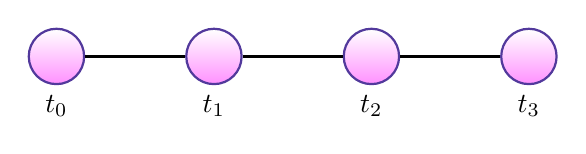
\begin{tikzpicture}[auto, thick]
  \node[time,label=below:$t_0$] (t0) at (0,0) {};
  \node[time,label=below:$t_1$] (t1) at (2,0) {};
  \node[time,label=below:$t_2$] (t2) at (4,0) {};
  \node[time,label=below:$t_3$] (t3) at (6,0) {};
  
  \path (t0) edge (t1);
  \path (t1) edge (t2);
  \path (t2) edge (t3);


\end{tikzpicture}
\caption{Multi-period optimal power flow example with four time-steps. The lines connecting the different time-periods denote the coupling between them.}
\label{fig:tcopflow}
\end{figure}


In general form, the equations for multi-period optimal power flow are given by
(\ref{eq:tcopflow_start}) -- (\ref{eq:tcopflow_end}). TCOPFLOW solves to minimize the total generation cost $\sum_{t=0}^{N_t-1}f(x_t)$ over the time horizon, where $N_t$ is the number of time-steps. At each time-step, the equality constraints ($g(x_t)$), inequality $h(x_t)$, and the lower/upper limit ($x^-$,$x^+$) constraints need to be satisfied. Equation (\ref{eq:tcopflow_end}) represents the coupling between the consecutive time-steps. It is a most common form of coupling that limits the deviation of the real power generation at time $t$ from its preceding time-step $t-\Delta{t}$ to within its ramping capability $\delta_t{x}$.


\begin{align}
\centering
\text{min}&~\sum_{t=0}^{N_t-1} f(x_t) &  \label{eq:tcopflow_start}\\
&\text{s.t.}& \nonumber \\
&~g(x_t) = 0,                                        &t \in \left[0,N_t-1\right]& \\
&~h(x_t) \le 0,                                      &t \in \left[0,N_t-1\right]& \\
x^- & \le x_t \le x^+,                               &t\in \left[0,N_t-1\right]& \\
-\delta_t{x} & \le x_t - x_{t-\Delta{t}} \le \delta_t{x},&t \in \left[1,N_t-1\right]&
\label{eq:tcopflow_end}
\end{align}

\section{Solvers}\label{sec:tcopflow_solvers}%
\tcopflow solves the coupled multi-period using the solver \ipopt. Currently, \exago only supports solving \tcopflow using \ipopt~, which is also the default solver. Solving TCOPFLOW is supported only on single process. %Option:\\ %\opflowoption{-tcopflow_solver IPOPT}

\section{Input and Output}
\begin{itemize}
    \item \textbf{Network file:} The network file describing the network details. Only \matpower format files are currently supported.
    \item \textbf{Load data:} One file for load real power and one fo reactive power. The files need to be in CSV format. An example of the format for the 9-bus case is \href{https://gitlab.pnnl.gov/exasgd/frameworks/exago/-/tree/master/datafiles/case9}{here}.
    \item \textbf{Wind generation:} The wind generation time-series described in CSV format. See an example of the format \href{https://gitlab.pnnl.gov/exasgd/frameworks/exago/-/tree/master/datafiles/case9}{here}.
\end{itemize}
If the load data and/or wind generation profiles are not set then a flat profile is assumed, i.e., the load and wind generation for all hours is constant.

The \tcopflow output is saved to a directory named \emph{tcopflowout}. This directory contains $N_t$ files, one for each time-step, in \matpower data file format.

\section{Usage}
\begin{lstlisting}
./tcopflow -netfile <netfilename> -tcopflow_pload_profile <ploadprofile> \
-tcopflow_windgen_profile <windgenprofile> <tcopflowoptions> \
-tcopflow_qload_profile <qloadprofile>
\end{lstlisting}
\section{Options}
See table \ref{tab:tcopflow_options}. In addition, all \opflow options given in Table \ref{tab:opflow_options} can be used.
\begin{table}[!htbp]
  \caption{TCOPFLOW options}
  \small
  \begin{tabular}{|p{0.4\textwidth}|p{0.3\textwidth}|p{0.3\textwidth}|}
    \hline
    \textbf{Option} & \textbf{Meaning} & \textbf{Values (Default value)} \\ \hline
    -netfile & Network file name & string (\href{https://gitlab.pnnl.gov/exasgd/frameworks/exago/-/blob/master/datafiles/case9/case9mod_gen3_wind.m}{case9mod\_gen3\_wind.m}) \\ \hline
    -save\_output & Save output to file & 0 or 1 (0) \\ \hline
    -tcopflow\_pload\_profile & Real power load profile & string (\href{https://gitlab.pnnl.gov/exasgd/frameworks/exago/-/blob/master/datafiles/case9/load_P.csv}{load\_P.csv}) \\ \hline
    -tcopflow\_qload\_profile & Reactive power load profile & string (\href{https://gitlab.pnnl.gov/exasgd/frameworks/exago/-/blob/master/datafiles/case9/load_Q.csv}{load\_Q.csv}) \\ \hline
    -tcopflow\_windgen\_profile & Wind generation profile & string (\href{https://gitlab.pnnl.gov/exasgd/frameworks/exago/-/blob/master/datafiles/case9/scenarios_9bus.csv}{case9/scenarios\_9bus.csv}) \\ \hline
    -tcopflow\_dT & Length of time-step (minutes) & double (5.0) \\ \hline
    -tcopflow\_duration & Total duration (hours) & double (0.5) \\ \hline 
    -tcopflow\_iscoupling & Coupling between time steps (ramp constraints) & 0 or 1 (0) \\ \hline
  \end{tabular}
  \label{tab:tcopflow_options}
\end{table}
\section{Examples}
Some \tcopflow example runs are provided with some sample output. Options are the default options provided in table \ref{tab:opflow_options} and \ref{tab:tcopflow_options} unless otherwise specified. Sample output is generated from running examples from the installation directory.

Example using \ipopt solver:

\begin{lstlisting}
$ ./bin/tcopflow -tcopflow_iscoupling 1 -print_output
[ExaGO INFO]: -- Checking ... -options_file not passed             exists: no
TCOPFLOW: Application created
TCOPFLOW: Duration = 0.500000 hours, timestep = 5.000000 minutes, \
                                     number of time-steps = 7
TCOPFLOW: Using IPOPT solver
TCOPFLOW: Setup completed
Setting: "0" is not a valid setting for Option: tol. 
Check the option documentation.

### tol (Real Number) ###
Category: Convergence
Description: Desired convergence tolerance (relative).
0 < (1e-08) <= +inf

*************************************************************************
This program contains Ipopt, a library for large-scale nonlinear 
optimization. Ipopt is released as open source code under the Eclipse 
Public License (EPL).
*************************************************************************

This is Ipopt version 3.12.10, running with linear solver ma27.

Number of nonzeros in equality constraint Jacobian...:      770
Number of nonzeros in inequality constraint Jacobian.:      610
Number of nonzeros in Lagrangian Hessian.............:      630

Total number of variables............................:      161
                     variables with only lower bounds:        0
                variables with lower and upper bounds:      105
                     variables with only upper bounds:        0
Total number of equality constraints.................:      126
Total number of inequality constraints...............:      186
        inequality constraints with only lower bounds:       42
   inequality constraints with lower and upper bounds:      144
        inequality constraints with only upper bounds:        0

iter  objective  inf_pr  inf_du lg(mu) ||d|| lg(rg) alpha_du alpha_pr  ls
0  5.2094875e+04 1.80e+00 5.02e+01  -1.0 0.00e+00 - 0.00e+00 0.00e+00   0
1  3.6277420e+04 1.40e+00 1.06e+02  -1.0 2.05e+00 - 1.88e-01 2.20e-01f  1
...
33  2.0843675e+04 1.13e-14 3.32e-09  -8.6 1.76e-08 - 1.00e+00 1.00e+00h 1

Number of Iterations....: 33

                                   (scaled)                 (unscaled)
Objective...........:   4.6734697780313832e+02    2.0843675210019970e+04
Dual infeasibility..:   3.3166774138882895e-09    1.4792381265941772e-07
Constraint violation:   1.1296519275560968e-14    1.1296519275560968e-14
Complementarity.....:   4.9900570925632554e-09    2.2255654632832121e-07
Overall NLP error...:   4.9900570925632554e-09    2.2255654632832121e-07


Number of objective function evaluations             = 47
Number of objective gradient evaluations             = 34
Number of equality constraint evaluations            = 47
Number of inequality constraint evaluations          = 47
Number of equality constraint Jacobian evaluations   = 34
Number of inequality constraint Jacobian evaluations = 34
Number of Lagrangian Hessian evaluations             = 33
Total CPU secs in IPOPT (w/o function evaluations)   =      0.025
Total CPU secs in NLP function evaluations           =      0.032

EXIT: Optimal Solution Found.
=============================================================
        Multi-Period Optimal Power Flow
=============================================================
OPFLOW Model                        POWER_BALANCE_POLAR
Solver                              IPOPT
Duration (minutes)                  30.00
Time-step (minutes)                 5.00
Number of steps                     7
Active power demand profile         datafiles/case9/load_P.csv
Rective power demand profile        datafiles/case9/load_Q.csv
Wind generation profile             datafiles/case9/scenarios_9bus.csv
Load loss allowed                   NO
Power imbalance allowed             NO
Ignore line flow constraints        NO

Number of variables                 168
Number of equality constraints      126
Number of inequality constraints    168
Number of coupling constraints      18

Convergence status                  CONVERGED
Objective value                     20843.68

----------------------------------------------------------------------
Bus        Pd      Qd      Vm      Va      mult_Pmis      mult_Qmis
----------------------------------------------------------------------
1         0.00    0.00   1.040   0.000      2063.35        -0.00
2         0.00    0.00   1.025   4.553      2013.40         0.00
3         0.00    0.00   1.025   2.955      2017.53         0.00
4         0.00    0.00   1.037  -2.174      2063.59        -0.74
5        75.00   30.00   1.025  -3.405      2074.28         2.68
6        90.00   30.00   1.023  -4.213      2092.22         4.26
7         0.00    0.00   1.033   0.783      2014.09         3.85
8       100.00   35.00   1.022  -1.667      2035.30         7.65
9         0.00    0.00   1.036   0.264      2018.00         3.11

--------------------------------------------------------------------------
From       To       Status     Sft      Stf     Slim     mult_Sf  mult_St
--------------------------------------------------------------------------
1          4          1       71.31    71.13   380.00    -0.00    -0.00
2          7          1      111.80   112.67   250.00    -0.00    -0.00
3          9          1       86.66    87.56   300.00    -0.00    -0.00
4          5          1       28.34    34.62   250.00    -0.00    -0.00
4          6          1       42.81    45.47   250.00    -0.00    -0.00
5          7          1       47.86    51.21   250.00    -0.00    -0.00
6          9          1       49.48    52.48   150.00    -0.00    -0.00
7          8          1       63.89    65.25   250.00    -0.00    -0.00
8          9          1       41.64    36.64   150.00    -0.00    -0.00

------------------------------------------------------------------------
Gen Status   Fuel     Pg       Qg       Pmin     Pmax     Qmin     Qmax
------------------------------------------------------------------------
1     1      COAL    71.06     5.89    10.00   350.00  -300.00   300.00
2     1      COAL   111.38    -9.71    10.00   300.00  -300.00   300.00
3     1      WIND    85.00   -16.87     0.00    85.00  -300.00   300.00
[ExaGO INFO]: Finalizing tcopflow application.
\end{lstlisting}

